\begin{solutionfigure}[htb]
    \centering
    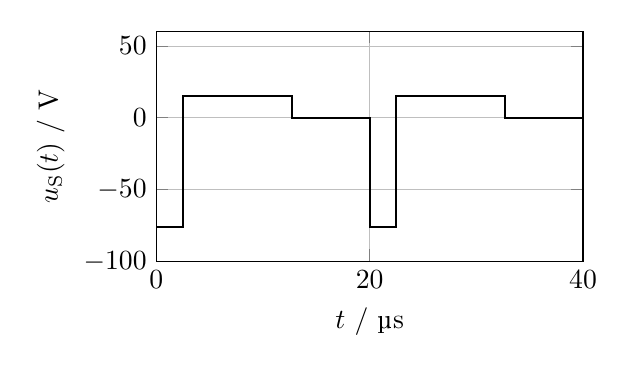
\begin{tikzpicture}
    \begin{axis}[
        width=7cm, height=4.5cm,
        grid=both,
        major grid style={line width=.2pt,draw=gray!50},
        minor grid style={line width=.1pt,draw=gray!20},
        xlabel={$t$ / µs},
        ylabel={$u_\mathrm{S}(t)$ / V},
       % title={$i_\mathrm{L}$ for minimum output power},
        xmin=0, xmax=40,
        ymin=-100, ymax=60,
        xtick={0, 20, 40},
        ytick={-100, -50, 0, 50},
        ]
        % Einschaltverhalten graph
        \addplot[
            thick,
            mark=none,
            color=black,
        ] coordinates {
            (0,0) (0,-76.4) (2.5,-76.4) (2.5, 15) (12.7, 15) (12.7, 0) (20, 0) (20, 0) (20, -76.4) (22.5, -76.4)(22.5, 15) (32.7, 15) (32.7, 0) (40, 0)
        };
    \end{axis}
    \end{tikzpicture} 
    \hspace{1cm} % Abstand zwischen den beiden Diagrammen
    \caption{Display of the voltage $u_\mathrm{S}(t)$.}
    \label{fig:voltageSecondarySideTask1}
    \end{solutionfigure}